\chapter[Anexos]{Anexos}
\section{Anexo A - Cronograma}

\begin{figure}[!h]
\centering
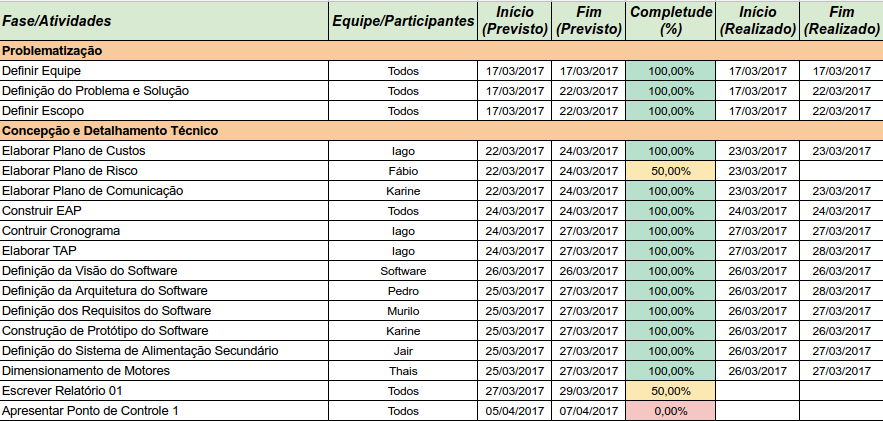
\includegraphics[scale=0.50, angle = 360]{figuras/cronograma1}
\caption[]{Cronograma Parte 01 (fonte: Autor)}
\end{figure}
\FloatBarrier

\begin{figure}[!h]
\centering
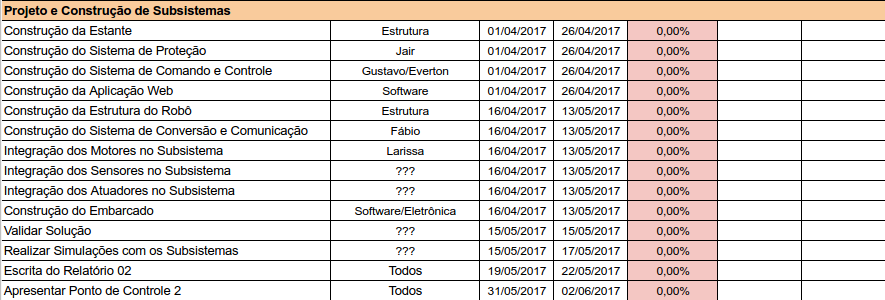
\includegraphics[scale=0.50, angle = 360]{figuras/cronograma2}
\caption[]{Cronograma Parte 02 (fonte: Autor)}
\end{figure}
\FloatBarrier

\begin{figure}[!h]
\centering
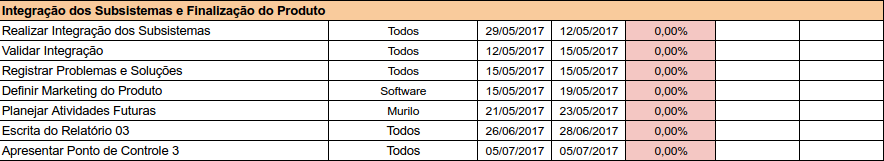
\includegraphics[scale=0.50, angle = 360]{figuras/cronograma3}
\caption[]{Cronograma Parte 03 (fonte: Autor)}
\end{figure}
\FloatBarrier

\section{Anexo B - Lista de atividades}

\begin{figure}[!h]
\centering
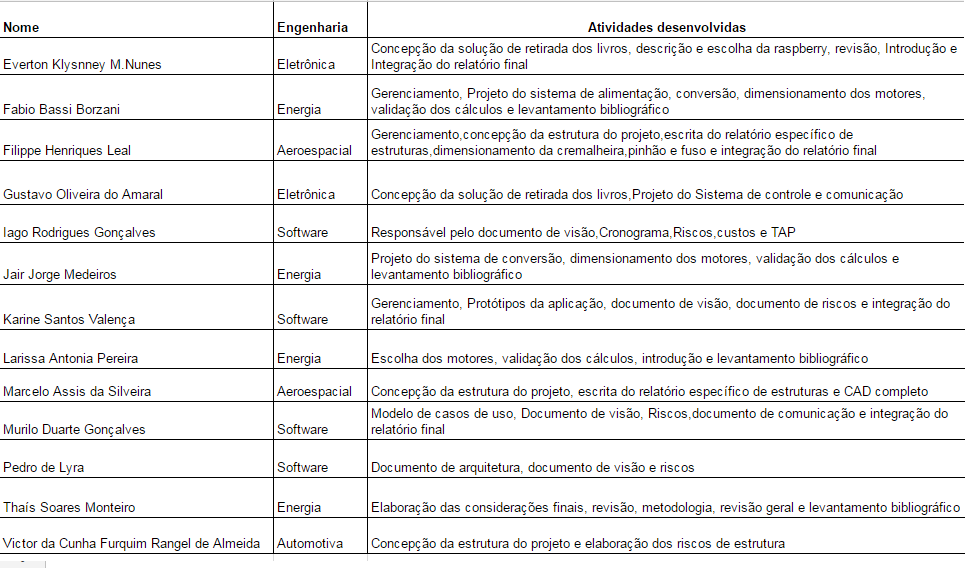
\includegraphics[scale=0.65, angle = 360]{figuras/lista_atividades}
\caption[]{Lista de atividades (fonte: Autor)}
\end{figure}
\FloatBarrier